\documentclass[12pt, answers]{exam}

% smaller margins
\usepackage[margin=1in, a4paper]{geometry}

% dfrac, therefore, because and others
\usepackage{mathtools}

% units
\usepackage{siunitx}

% diagrams, graphs
\usepackage{tikz, pgfplots}
\pgfplotsset{compat=1.18}

% line spacing
\usepackage{setspace}

% cancellation
\usepackage{cancel}

% cases
\usepackage{cases}

% labelling
\usepackage[nolabel, final]{showlabels}

% font
\usepackage[T1]{fontenc}
\usepackage[lf]{MinionPro}

% make life easier
\newcommand{\reals}{\mathbb{R}}
\newcommand{\ints}{\mathbb{Z}}
\newcommand{\posints}{\mathbb{Z}^{+}}
\newcommand{\rationals}{\mathbb{Q}}
\newcommand{\complexes}{\mathbb{C}}
\renewcommand{\frac}[2]{\dfrac{#1}{#2}}

\pagestyle{plain}

\begin{document}
\onehalfspacing%

\begin{center}
	\Large
	\textbf{Problem Of The Day 2022}
\end{center}

\begin{questions}
	\question (\textbf{21 Mar}) Simplify the algebraic fraction
	\( \frac{a^4-a^2b^2}{(a-b)^2} \div \frac{a(a+b)}{b^2} \times \frac{b}{a} \).

	\begin{solution}
		\begin{align*}
			 & \frac{a^4-a^2b^2}{(a-b)^2} \div \frac{a(a+b)}{b^2} \times \frac{b}{a}                                               \\
			 & = \frac{\cancel{a^2(a+b)(a-b)}}{(a-b)^{\cancel{2}}} \times\frac{b^{2}}{\cancel{a(a+b)}} \times \frac{b}{\cancel{a}} \\
			 & = \frac{b^3}{a-b}
		\end{align*}
	\end{solution}

	\question (\textbf{22 Mar}) Factorise \(a^4+a^2b^2+b^2\).
	\begin{solution}
		\begin{align*}
			a^4 + a^2b^2 + b^4 & = a^4 + 2a^2b^2 + b^4 - a^2b^2     \\
			                   & = (a^2 + b^2)^2 - (ab)^2           \\
			                   & = (a^2 - ab + b^2)(a^2 + ab + b^2)
		\end{align*}
	\end{solution}

	\question (\textbf{23 Mar}) Simplify \(\frac{1}{a-x}-\frac{1}{a+x}-\frac{2x}{a^2+x^2}-\frac{4x^3}{a^4+x^4}+\frac{8x^7}{a^8-x^8}\).
	\begin{solution}
		\begin{align*}
			 & \frac{1}{a-x}-\frac{1}{a+x}-\frac{2x}{a^2+x^2}-\frac{4x^3}{a^4+x^4}+\frac{8x^7}{a^8-x^8} \\
			 & = \frac{2x}{a^2-x^2}-\frac{2x}{a^2+x^2}-\frac{4x^3}{a^4+x^4}+\frac{8x^7}{a^8-x^8}        \\
			 & = \frac{4x^3}{a^4-x^4}-\frac{4x^3}{a^4+x^4}+\frac{8x^7}{a^8-x^8}                         \\
			 & = \frac{8x^7}{a^8-x^8}+\frac{8x^7}{a^8-x^8}                                              \\
			 & = \frac{16x^7}{a^8-x^8}
		\end{align*}
	\end{solution}

	\question (\textbf{24 Mar}) Factorise completely
	\(64x^6 - y^{12}\).
	\begin{solution}
		\begin{align*}
			64x^6 - y^{12} & = (8x^3 + y^6)(8x^3 - y^6)                                     \\
			               & = (2x + y^2)(2x - y^2)(4x^2 + 2xy^2 + y^4)(4x^2 - 2xy^2 + y^4) \\
		\end{align*}
	\end{solution}

	\question (\textbf{25 Mar}) Factorise completely \(x^2(x-1)^2 + 32(x-x^2) + 60\).
	\begin{solution}
		\begin{align*}
			 & x^2(x-1)^2 + 32(x-x^2) + 60             \\
			 & = x^2(x-1)^2 - 32x(x-1) + 60            \\
			 & = [x(x-1)]^2 - 32[x(x-1)] + 16^2 - 14^2 \\
			 & = [x(x-1) - 16]^2 - 14^2                \\
			 & = (x^2-x-2)(x^2-x-30)                   \\
			 & = (x-6)(x-2)(x+1)(x+5)
		\end{align*}
	\end{solution}

	\question (\textbf{28 Mar}) Simplify
	\(\frac{x^2-4}{x^2-4x+4}+\frac{2-x}{x+2}\).
	\begin{solution}
		\begin{align*}
			 & \frac{x^2-4}{x^2-4x+4} + \frac{2-x}{x+2}                              \\
			 & = \frac{(x+2)\cancel{(x-2)}}{(x-2)^{\cancel{2}}} + \frac{-(x-2)}{x+2} \\
			 & = \frac{(x+2)^2 - (x-2)^2}{(x+2)(x-2)}                                \\
			 & = \frac{8x}{x^2 - 4}
		\end{align*}
	\end{solution}

	\question (\textbf{29 Mar}) An equation in \(x\),
	\(\frac{m}{x-1} + \frac{3}{1-x} = 1\), has a positive solution.
	Find the possible range of values for \(m\).
	\begin{solution}
		\begin{align*}
			\frac{m}{x-1} + \frac{3}{1-x} & = 1     \\
			m - 3                         & = x - 1 \\
			x                             & = m - 2 \\
			\because x                    & > 0     \\
			\therefore m                  & > 2     \\
		\end{align*}
	\end{solution}

	\question (\textbf{30 Mar}) Given that \(\frac{1}{x} + \frac{1}{y} = 3\),
	find the value of \(\frac{3x + 4xy + 3y}{x + 2xy + y}\).
	\begin{solution}
		\begin{align*}
			\because \frac{1}{x} + \frac{1}{y} & = 3                                                            \\
			\therefore x + y                   & = 3xy                                                          \\
			\\
			\frac{3x+4xy+3y}{x+2xy+y}          & = \frac{\frac{13}{3}\cancel{(x+y)}}{\frac{5}{3}\cancel{(x+y)}} \\
			                                   & = \frac{13}{5}                                                 \\
		\end{align*}
	\end{solution}

	\question (\textbf{31 Mar})
	A factory scheduled to manufacture 480 toys within a number of days.
	The factory increased its daily production by 50\% since the beginning
	of the production and finished the whole batch of 480 toys 10 days earlier
	than the original schedule. How many toys per day did the factory plan
	to manufacture originally?

	\begin{solution}
		Let \(x\) be the number of toys per day the factory planned to manufacture originally.
		\begin{align*}
			\frac{480}{x} - \frac{480}{\frac{3}{2}x} & = 10    \\
			\frac{720x - 480x}{\frac{3}{2}x^2}       & = 10    \\
			240x                                     & = 15x^2 \\
			x                                        & = 16
		\end{align*}
		The company originally planned to manufacture 16 toys per day.
	\end{solution}

	\question (\textbf{1 Apr})
	Make \(y\) the subject of the formula:
	\[\sqrt{\frac{x^3-x+y}{xy}} = x\]
	\begin{solution}
		\begin{align*}
			\sqrt{\frac{x^3-x+y}{xy}} & = x                                                    \\
			x^2                       & = \frac{x^3-x+y}{xy}                                   \\
			x^3y                      & = x^3-x+y                                              \\
			y(x^{3}-1)                & = x^{3}-x                                              \\
			y                         & = \frac{x^{3}-x}{x^{3}-1}                              \\
			                          & = \frac{x(x+1)\cancel{(x-1)}}{\cancel{(x-1)}(x^2+x+1)} \\
			                          & = \frac{x(x+1)}{x^2+x+1}
		\end{align*}
	\end{solution}

	\question (\textbf{4 Apr}) Solve the SLEs:
	\begin{numcases}{}
		\frac{1}{x} + \frac{1}{y} & = 5     \\
		xy                          & = \(x - y\)
	\end{numcases}
	\begin{solution}
		\begin{align*}
			\text{From (1):}                                     &                                                                                               \\
			xy                                                   & = \frac{x+y}{5} \text{\quad(3)}                                                               \\
			\text{Substitute (3) into (2):}                      &                                                                                               \\
			x+y                                                  & = 5x - 5y                                                                                     \\
			4x                                                   & = 6y                                                                                          \\
			x                                                    & = \frac{3}{2}y \text{\quad(4)}                                                                \\
			\text{Substitute (4) into (2):}                      &                                                                                               \\
			\frac{3}{2}y^{2}                                     & = \frac{1}{2}y                                                                                \\
			y\left(\frac{3}{2}y-\frac{1}{2}\right)               & = 0                                                                                           \\
			\therefore y                                         & = 0 \left(\text{rej., } \frac{1}{y} \text{ cannot be undefined}\right) \text{or } \frac{1}{3} \\
			\text{Substitute } y = \frac{1}{3} \text{ into (2):} &                                                                                               \\
			\frac{1}{3}x                                         & = x - \frac{1}{3}                                                                             \\
			\frac{2}{3}x                                         & = \frac{1}{3}                                                                                 \\
			x                                                    & = \frac{1}{2}                                                                                 \\
			\therefore x                                         & = \frac{1}{2} \text{ and } y = \frac{1}{3}
		\end{align*}
	\end{solution}

	\question (\textbf{5 Apr})
	\begin{parts}
		\part Find the equation of the line \(l_{1}\) that makes a \ang{45} angle with the positive \(x\)-axis and its \(y\)-intercept is \(-3\).
		\begin{solution}
			Since the angle between the positive \(x\)-axis and \(l_{1}\) has to be \ang{45}, the gradient (\(m\)) can only be \(1\).
			Since the \(y\)-intercept is \(-3\), the value of \(c\) in the gradient-intercept form has to be \(-3\) as well.
			Therefore, the equation of line \(l_{1}\) is \(y = x - 3\).
		\end{solution}

		\part Hence, find the equation of a vertical line \(l_{2}\) which
		intersects with \(l_{1}\) at a point with a \(y\)-coordinate of 10.
		\begin{solution}
			\begin{align*}
				y            & = x - 3 \\
				10           & = x - 3 \\
				\therefore x & = 13
			\end{align*}
			The equation of line \(l_{2}\) is \(x = 13\).
		\end{solution}

		\part Are the following three points collinear:
		the intersection point between \(l_{1}\) and \(l_{2}\),
		the origin, and \((-6.5, -5)\)?
		\begin{solution}
			There can be a line, \(l_{3}\), with both the origin and the intersection on it.
			The equation of this line would thus be:
			\begin{equation*}
				y = \frac{10 - 0}{13 - 0}x = \frac{10}{13}x
			\end{equation*}
			Substituting \(x = -6.5\) and \(y = -5\) into that equation,
			we see that:
			\[
				-5 = \frac{10}{13} \times -\frac{13}{2}
			\]
			Therefore, all three points are collinear.
		\end{solution}
	\end{parts}

	\question (\textbf{7 Apr}) Expand and simplify the expression \(\left[x\left(x^{4}-y^{4}\right)-3xy\left(-y\right)^{3}\right] \cdot x^{2}y\).
	\begin{solution}
		\begin{align*}
			 & \left[x\left(x^{4}-y^{4}\right)-3xy\left(-y\right)^{3}\right] \cdot x^{2}y \\
			 & = x^{3}y\left[x^{4}-y^{4}-3y\left(-y\right)^{3}\right]                     \\
			 & = x^{3}y\left(x^{4}+2y^{4}\right)
		\end{align*}
	\end{solution}

	\question (\textbf{8 Apr}) There is a rectangular piece of paper
	with length \((5a + 4b)\) and breadth \((4a + 3b)\). A square of
	side length \((a + b)\) is cut away from the four corners of the
	paper. Using the remaining paper, a box without its top cover
	can be folded.
	\begin{parts}
		\part Find the total surface area of the folded paper box.
		\begin{solution}
			Draw the diagram.

			\begin{tikzpicture}
				\draw [red, dashed] (0, 0) -- node[below] {\(a + b\)} (2, 0);
				\draw [red, dashed] (0, 0) -- (0, 2);
				\draw (0, 2) -- (2, 2);
				\draw (2, 2) -- (2, 0);
				\draw (0, 2) -- (0, 6);
				\draw (0, 6) -- (2, 6);
				\draw [blue, dashed] (2, 6) -- node[right] {\(2a + b\)} (2, 2);
				\draw [red, dashed] (0, 6) -- (0, 8);
				\draw [red, dashed] (0, 8) -- (2, 8);
				\draw (2, 8) -- (2, 6);
				\draw (2, 8) -- node[above] {\(5a + 4b\)} (8, 8);
				\draw [latex-](0, 8.25) -- (4.25, 8.25);
				\draw [-latex](5.75, 8.25) -- (10, 8.25);
				\draw (8, 8) -- (8, 6);
				\draw [blue, dashed] (8, 6) -- (8, 2);
				\draw (8, 6) -- (10, 6);
				\draw (10, 6) -- node[right] {\(4a + 3b\)}( 10, 2);
				\draw [-latex](10.25, 4.25) -- (10.25, 8);
				\draw [-latex](10.25, 3.75) -- (10.25, 0);
				\draw (10, 2) -- (8, 2);
				\draw (8, 2) -- (8, 0);
				\draw (8, 0) -- (2, 0);
				\draw [magenta, dashed] (8, 2) -- node[above] {\(3a + 2b\)}(2, 2);
				\draw [magenta, dashed] (8, 6) -- (2, 6);
				\draw [red, dashed] (8, 8) -- (10, 8);
				\draw [red, dashed] (10, 8) -- (10, 6);
				\draw [red, dashed] (10, 2) -- (10, 0);
				\draw [red, dashed] (10, 0) -- (8, 0);
			\end{tikzpicture}

			\begin{align*}
				\text{total surface area}
				 & = 2 \cdot \left[\left(5a + 4b\right)\left(4a+3b\right) - 4(a+b)\right] \\
				 & = 2\left(20a^{2}+15ab+16ab+12b^{2}-4\left(a+b\right)\right)            \\
				 & = 40a^{2} + 62ab + 24b^{2} - 8a - 8b
			\end{align*}
		\end{solution}
		\part Find the volume of the paper box.
		\begin{solution}
			\begin{align*}
				\text{volume of paper box} & = (3a+2b)(2a+b)(a+b)                   \\
				                           & = 6a^{3} + 13a^{2}b + 9ab^{2} + 2b^{3}
			\end{align*}
		\end{solution}
	\end{parts}

	\question (\textbf{11 Apr}) Solve the equation
	\((x+1)(1-3x)(4y-5) = 7(5-4y)\).
	\begin{solution}
		\\
		\textbf{Case 1}: Solve for \(x\).
		\begin{align*}
			(x+1)(1-3x)\cancel{(4y-5)}      & = -7\cancel{(4y-5)} \\
			-3x^{2}	- 2x + 1 + 7            & = 0                 \\
			(-3x + 4)(x + 2)                & = 0                 \\
			\therefore x = -2 \text{ or } x & = \frac{4}{3}
		\end{align*}

		Both possibilities of \(x\) in \textbf{Case 1} result
		in an identity when trying to solve for \(y\), so we can say
		when \(x = -2\) or \(\frac{4}{3}\), \(y \in \reals\).

		\textbf{Case 2}: Solve for \(y\).
		\begin{align*}
			(x+1)(1-3x)(4y-5)                        & = 7(5-4y)                                        \\
			-12x^{2}y + 15x^{2} - 8xy + 10x + 4y - 5 & = -28y + 35                                      \\
			y \left(-12x^{2} - 8x + 32 \right)       & = -15x^{2} - 10x + 40                            \\
			y                                        & = \frac{-15x^{2} - 10x + 40}{-12x^{2} - 8x + 32} \\
			                                         & = \frac{5}{4}
		\end{align*}
		The solution \(y = \frac{5}{4}\) results in an identity
		when trying to solve for \(x\), so we can also say that when
		\(y = \frac{5}{4}\), \(x \in \reals\).

		\[
			\therefore
			\begin{cases}
				x = -2 \text{ or } \frac{4}{3}, & y \in \reals    \\
				x \in \reals,                   & y = \frac{5}{4}
			\end{cases}
		\]
	\end{solution}

	\question(\textbf{12 Apr}) Out of the following equations:
	\[2x^{2} + x - 3\]
	\[\frac{5x}{x^{2} + 1} = 2\]
	\[ (x + 1)(x - 2) = x^{2} \]
	\[ \left(t + 1\right)^{2} = 2t(t + 1) \]
	How many quadratic equations are there?
	\begin{solution}
		There are \textbf{2} quadratic equations.
		\begin{enumerate}
			\item	\(2x^{2} + x - 3\) is an expression, not an equation.
			\item \(\frac{5x}{x^{2} + 1}\) can be expressed in the form \(ax^{2} + bx + c = 0\).
			      \begin{align*}
				      \frac{5x}{x^{2} + 1} & = 2                       \\
				      5x                   & = 2\left(x^{2} + 1\right) \\
				      2x^{2} - 5x + 2      & = 0
			      \end{align*}
			\item \((x + 1)(x - 2) = x^{2}\) cannot be expressed in the form \(ax^{2} + bx + c = 0\). It is in fact, a linear equation.
			      \begin{align*}
				      (x + 1)(x - 2) & = x^{2} \\
				      x^{2} - x - 2  & = x^{2} \\
				      -x - 2         & = 0
			      \end{align*}
			\item \(\left(t + 1\right)^{2} = 2t(t + 1)\) can be expressed in the form \(ax^{2} = c\).
			      \begin{align*}
				      \left(t + 1\right)^{2}  & = 2t(t + 1)            \\
				      t^{2} + \cancel{2t} + 1 & = 2t^{2} + \cancel{2t} \\
				      t^{2}                   & = 1
			      \end{align*}
		\end{enumerate}
	\end{solution}

	\question (\textbf{13 Apr})
	For an equation in \(x\), \(\left(m^{2} - 8m + 17\right)x^{2} - 2mx + 1 = 0\), where \(m\) is a real constant.
	Which of the following statements is true?

	\begin{choices}
		\choice It is a quadratic equation.
		\choice It is a linear equation.
		\choice It cannot be determined if it is a quadratic equation.
	\end{choices}

	\begin{solution}
		\textbf{C}.

		Although it is true that \(m^{2} - 8m + 17 \in \reals\) and \(-2m \in \reals\),
		which makes the equation seem to conform to the standard form of
		\(ax^{2} + bx + c = 0\), there is a possibility that
		\(m^{2} - 8m + 17 = 0\), which makes the \(ax^{2}\) term \(0\),
		causing the equation to no longer be quadratic. Due to the value of \(m\) being unknown, we cannot confirm
		whether the equation is quadratic.
	\end{solution}

	\question (\textbf{14 Apr}) Solve the quadratic equation
	\((x - 1)^{2} - 5x(x + 5) = -2(x - 2) + 3\).
	\begin{solution}
		\begin{align*}
			(x - 1)^{2} - 5x(x + 5)                          & = -2(x - 2) + 3              \\
			x^{2} - 2x + 1 - 5x^{2} - 25x                    & = -2x + 7                    \\
			-4x^{2} - 25x - 6                                & = 0                          \\
			\left(-4x^{2} - x\right) + \left(-24x - 6\right) & = 0                          \\
			(4x + 1)(- x - 6)                                & = 0                          \\
			\therefore x                                     & = -6 \text{ or} -\frac{1}{4}
		\end{align*}
	\end{solution}

	\question (\textbf{18 Apr}) A rectangle of breadth \qty{2}{\centi\metre} is cut from a square.
	The rectangle's length is the same as the square's.
	The remaining area is \qty{48}{\square\centi\metre}.
	Find the original area of the square.
	\begin{solution}
		Let the length of the square be \(x\) \si{\centi\metre}.
		\begin{align*}
			x^{2} - 2x                  & = 48 \\
			(x + 6)(x - 8)              & = 0  \\
			x = -6 \text{ (rej.) or } x & = 8  \\
			\therefore  x^{2}           & = 64
		\end{align*}
		The original area of the square is \qty{64}{\square\centi\metre}.
	\end{solution}

	\question (\textbf{19 Apr}) Determine if the following relationships are quadratic functions.
	\begin{parts}
		\part Within a certain distance, the speed of the train \(v\) \si{\kilo\metre\per\hour} and the time \(t\) \si{\hour}.
		\begin{solution}
			No. Both \(v\) and \(t\) are constants within that certain distance.
		\end{solution}

		\part The perimeter \(C\) and the length of the side \(a\) of an equilateral triangle.
		\begin{solution}
			No. \(C = 3a\).
		\end{solution}

		\part The area \(S\) and the length of radius \(R\) of a sector of angle \ang{120}.
		\begin{solution}
			Yes. \(S = \frac{1}{3} \pi r^{2}\).
		\end{solution}
	\end{parts}

	\question (\textbf{20 Apr}) There is a \qty{56}{\centi\metre} piece of wire.
	It is cut into two pieces and each piece is then made into a square.
	\begin{parts}
		\part If the sum of the areas of the two squares is \qty{100}{\square\centi\metre},
		how should the wire be cut?
		\begin{solution}
			Let the lengths of the two pieces be \(x\) \si{\centi\metre} and \(y\) \si{\centi\metre} respectively.
			\begin{align}
				x + y                                                          & = 56 \label{eq:0420a1} \tag{1}  \\
				{\left(\frac{x}{4}\right)}^{2}+ {\left(\frac{y}{4}\right)}^{2} & = 100 \label{eq:0420a2} \tag{2}
			\end{align}
			From \eqref{eq:0420a2}:
			\begin{align*}
				\frac{x^{2} + y^{2}}{16} & = 100                            \\
				x^{2} + y^{2}            & = 1600 \label{eq:0420a3} \tag{3} \\
			\end{align*}
			Substitute \eqref{eq:0420a1} into \eqref{eq:0420a3}:
			\begin{align*}
				x^{2} + (56 - x)^{2}        & = 1600                                        \\
				x^{2} + 3136 - 112x + x^{2} & = 1600                                        \\
				2x^{2}  - 112x + 1536       & = 0                                           \\
				x^{2}  - 56x + 768          & = 0                                           \\
				(x - 24)(x - 32)            & = 0                                           \\
				x                           & = 24 \text{ or } 32 \label{eq:0420a4} \tag{4} \\
			\end{align*}
			Substitute \eqref{eq:0420a4} into \eqref{eq:0420a1}:
			\[
				\begin{cases}
					x = 24, y = 32 \\
					x = 32, y = 24 \\
				\end{cases}
			\]
			Hence, the wire should be cut into \qty{24}{\centi\metre} and \qty{32}{\centi\metre} pieces.
		\end{solution}

		\part If the sum of the areas of the two squares is \qty{196}{\square\centi\metre},
		how should the wire be cut?
		\begin{solution}
			Let the lengths of the two pieces be \(x\) \si{\centi\metre} and \(y\) \si{\centi\metre} respectively.
			\begin{align}
				x + y                                                          & = 56 \label{eq:0420b1} \tag{1}  \\
				{\left(\frac{x}{4}\right)}^{2}+ {\left(\frac{y}{4}\right)}^{2} & = 196 \label{eq:0420b2} \tag{2}
			\end{align}
			From \eqref{eq:0420b2}:
			\begin{align*}
				\frac{x^{2} + y^{2}}{16} & = 196                            \\
				x^{2} + y^{2}            & = 3136 \label{eq:0420b3} \tag{3} \\
			\end{align*}
			Substitute \eqref{eq:0420b1} into \eqref{eq:0420b3}:
			\begin{align*}
				x^{2} + (56 - x)^{2}        & = 3136                    \\
				x^{2} + 3136 - 112x + x^{2} & = 3136                    \\
				2x^{2}  - 112x              & = 0                       \\
				x^{2}  - 56x                & = 0                       \\
				x( x - 56 )                 & = 0                       \\
				x                           & = 0 \text{ (rej.) or } 56
			\end{align*}
			Hence, the wire cannot be cut into two such pieces.
		\end{solution}

		\part Is it possible for the sum of the two areas to be \qty{200}{\square\centi\metre}?
		\begin{solution}
			Assuming that it \textbf{is} possible:

			Let the lengths of the two pieces be \(x\) \si{\centi\metre} and \(y\) \si{\centi\metre} respectively.
			\begin{align}
				x + y                                                          & = 56 \label{eq:0420c1} \tag{1}  \\
				{\left(\frac{x}{4}\right)}^{2}+ {\left(\frac{y}{4}\right)}^{2} & = 200 \label{eq:0420c2} \tag{2}
			\end{align}
			From \eqref{eq:0420c2}:
			\begin{align*}
				\frac{x^{2} + y^{2}}{16} & = 200                            \\
				x^{2} + y^{2}            & = 3200 \label{eq:0420c3} \tag{3} \\
			\end{align*}
			Substitute \eqref{eq:0420c1} into \eqref{eq:0420c3}:
			\begin{align*}
				x^{2} + (56 - x)^{2}        & = 3200                         \\
				x^{2} + 3136 - 112x + x^{2} & = 3200                         \\
				2x^{2}  - 112x - 64         & = 0                            \\
				x^{2}  - 56x -32            & = 0                            \\
				x                           & = \frac{56 \pm \sqrt{3264}}{2} \\
			\end{align*}
			Even if we reject the negative case, \(x = \frac{56 - \sqrt{3264}}2\),
			\(y\) will still be negative,
			rendering it impossible for the sum of the areas of the two squares to be \qty{200}{\square\centi\metre}.
		\end{solution}
	\end{parts}

	\question (\textbf{21 Apr}) The graph of a quadratic function
	\(y = mx^2 + x + m(m - 2)\) passes through the origin. Find the value of \(m\).
	\begin{solution}
		Substituting \(x = 0\) and \(y = 0\) into the equation:
		\begin{align*}
			0            & = m \cdot 0^{2} + 0 + m(m - 2) \\
			m(m - 2)     & = 0                            \\
			m            & = 0 \text{ (rej.) or } 2       \\
			\therefore m & = 2
		\end{align*}
	\end{solution}

	\question (\textbf{22 Apr}) Refer to the quadratic graph below.
	Which of the following could be the equation of said graph?
	\begin{figure}[htpb]
		\centering
		\begin{tikzpicture}
			\begin{axis}[
					domain=-5:7,
					axis x line=middle,
					axis y line=middle,
					xlabel=\(x\),
					ylabel=\(y\),
					ticks=none,
					ymax=5,
				]
				\addplot[black, thick] {-x^2 + 2 * x + 3};
			\end{axis}
		\end{tikzpicture}
		\label{fig:0422}
	\end{figure}
	\begin{choices}
		\choice \(y = x^{2} - 2x + 3\)
		\choice \(y = -x^{2} - 2x + 3\)
		\choice \(y = x^{2} + 2x + 3\)
		\choice \(y = -x^{2} + 2x + 3\)
	\end{choices}
	\begin{solution}
		\textbf{D}.

		The graph is a `n'-shaped one, meaning the coefficient of the \(x^{2}\) term is negative.
		The turning point of the curve is also within the positive \(x\)-axis, so the coefficient
		of the \(x\) term is positive, leaving the option of \textbf{D}.
	\end{solution}

	\question (\textbf{25 Apr}) If \(\left(-\frac{13}{4}, y_{1}\right)\), \(\left(-1, y_{2}\right)\), \(\left(\frac{5}{3}, y_{3}\right)\)
	are three points on a quadratic curve with equation \(y = -x^{2} - 4x + 5\),
	which of the following is true?

	\begin{oneparchoices}
		\choice \(y_{1} < y_{2} < y_{3}\)
		\choice \(y_{3} < y_{2} < y_{1}\)
		\choice \(y_{3} < y_{1} < y_{2}\)
		\choice \(y_{2} < y_{1} < y_{3}\)
	\end{oneparchoices}
	\begin{solution}
		\textbf{C}.
		\begin{itemize}
			\item The graph is a `n'-shaped one as the coefficient of the \(x^{2}\) term is negative.
			\item The maximum point is on the negative \(x\)-axis as the coefficient of the \(x\) term is negative. It lies on the line \(x = -2\).
			\item The coordinates of \(x\)-intercepts are \num{1} and \num{-5}.
			      \begin{align*}
				      0               & = -x^{2} - 4x + 5  \\
				      (-x + 1)(x + 5) & = 0                \\
				      x               & = 1 \text{ or } -5
			      \end{align*}
		\end{itemize}
		\textbf{Conclusions}:
		\begin{itemize}
			\item \(y_{2}\) is the largest as its point's \(x\)-coordinate is the closest to the maximum point.
			\item The point with \(y\)-coordinate \(y_{1}\) is in the 2nd Quadrant.
			\item \(y_{3} < y_{1} < y_{2}\).
		\end{itemize}
	\end{solution}

	\question (\textbf{26 Apr}) Refer to the graph of the quadratic function, \(y = ax^2 + bx + c \) below,
	where \(a \neq 0\). Which of the following statement(s) is / are correct?
	\begin{figure}[htpb]
		\centering
		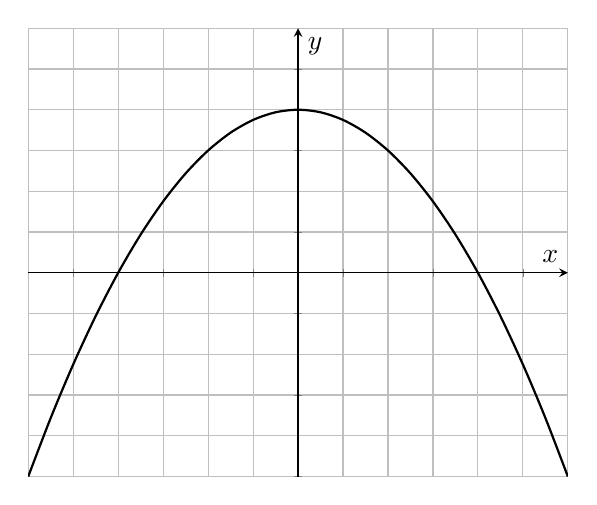
\begin{tikzpicture}
			\begin{axis}[
					domain=-3:3,
					axis x line=middle,
					axis y line=middle,
					xlabel=\(x\),
					ylabel=\(y\),
					grid=both,
					no markers,
					smooth,
					minor tick num=1,
					ticks=none,
					ymax=6,
				]
				\addplot[black, thick] {-x^2 + 4};
			\end{axis}
		\end{tikzpicture}
	\end{figure}

	\begin{oneparchoices}
		\choice \(a > 0\)
		\choice \(c > 0\)
		\choice \(\frac{a}{c} > 0\)
		\choice \(-ac < 0\)
	\end{oneparchoices}

	\begin{solution}
		\textbf{B}.
		\begin{enumerate}
			\item The graph is an `n'-shaped one, so \(a < 0\).
			\item The graph intercepts the \(y\)-axis on the positive \(y\)-axis, so \(c > 0\).
			\item Since \(a < 0\) and \(c > 0\), \(\frac{a}{c} < 0\).
			\item Since \(a < 0\) and \(c > 0\), \(-ac > 0\).
		\end{enumerate}
	\end{solution}

	\question (\textbf{27 Apr}) Refer to the graph of the quadratic function, \(y = ax^2 + bx + c \) below,
	where \(a \neq 0\). The line of symmetry passes through \((1, 0)\).
	Which of the following statement(s) is/are correct?
	\begin{figure}[htpb]
		\centering
		\begin{tikzpicture}
			\begin{axis}[
					domain=-3:5,
					smooth,
					axis x line=middle,
					axis y line=middle,
					xlabel=\(x\),
					ylabel=\(y\),
					% grid=both,
					xtick={-1, 1},
					ytick=\empty,
					ymin=-5,
					ymax=4,
				]
				\addplot[black, thick] {-x^2 + 2 * x + 2};
				\addplot[red, thick, dashed] coordinates{(1,10) (1,-25)};
			\end{axis}
		\end{tikzpicture}
	\end{figure}

	\begin{oneparchoices}
		\choice \(abc > 0\)
		\choice \(b > a + c\)
		\choice \(a + b + c < 0\)
	\end{oneparchoices}

	\begin{solution}
		\textbf{B}.
		\begin{enumerate}
			\item The graph is an `n'-shaped one, so \(a < 0\).
			      The turning point is on the positive side of the \(x\)-axis, so \(b > 0\).
			      The \(y\)-intercept is on the positive \(y\)-axis, so \(c > 0\).
			      \(\therefore abc < 0\).
			\item \(b > a + c \Rightarrow a - b + c < 0\).
			      Substituting the values of \(x = -1\) into \(y = ax^2 + bx + c\)
			      returns \(y = a - b + c\). The point on the curve with \(x\)-coordinate \num{-1}
			      has a negative \(y\)-coordinate, hence \(y < 0 \Rightarrow a - b + c < 0 \Rightarrow b > a + c\).
			\item At the maximum point, \((x_P, y_P)\), \(y_P > 0\). Since \(x_P = 1\),
			      \(a{x_P}^2 + bx_P + c = a + b + c = y_P\), so \(a + b + c > 0\).
		\end{enumerate}
	\end{solution}


	\question (\textbf{28 Apr}) Refer to the graph of the quadratic function
	below, where the equation of the function is \(y = ax^2 + bx + c\), \(a \neq 0\).
	Which of the following statement(s) is/are correct?
	\begin{figure}[htpb]
		\centering
		\begin{tikzpicture}
			\begin{axis}[
					axis lines=middle,
					xlabel= $x$,
					ylabel= $y$,
					ticks = none,
					scaled ticks = false,
					xmin = -3,
					xmax = 6,
					ymin = -30,
					ymax = 2,
				]
				\addplot[
					black,
					thick,
					domain = -3:6,
					smooth,
				] {-x^2 + 3 * x - 6};
			\end{axis}
		\end{tikzpicture}
	\end{figure}

	\begin{oneparchoices}
		\choice \(ab > 0\)
		\choice \(abc > 0\)
		\choice \(a - b + c > 0\)
		\choice \(a + b + c < 0\)
	\end{oneparchoices}

	\begin{solution}
		\textbf{B} and \textbf{D}.
		\begin{enumerate}
			\item \(a < 0\) since the graph is `n'-shaped, and \(b > 0\) since the turning point is on the positive \(x\)-axis. \(\therefore ab < 0\).
			\item \(a < 0\) and \(b > 0\). \(c < 0\) since the graph intercepts the \(y\)-axis on the negative \(y\)-axis. \(\therefore abc > 0\).
			\item \(a < 0\), \(b > 0\) and \(c < 0\), \(\therefore a - b + c < 0\).
			\item We can assume that the point with an \(x\)-coordinate of \num{1}
			      (which is greater than 0), lies on the negative \(y\)-axis. Substituting
			      \(x = 1\) into \(y = ax^2 + bx + c\) would yield \(y = a + b + c\). Indeed,
			      \(y < 0\) for such a point, hence \(a + b + c < 0\).
		\end{enumerate}
	\end{solution}

	\question (\textbf{29 Apr}) The graph of the quadratic function \(y = 3x^{2} + 4x + 1\) is shown below.
	\begin{figure}[htpb]
		\centering
		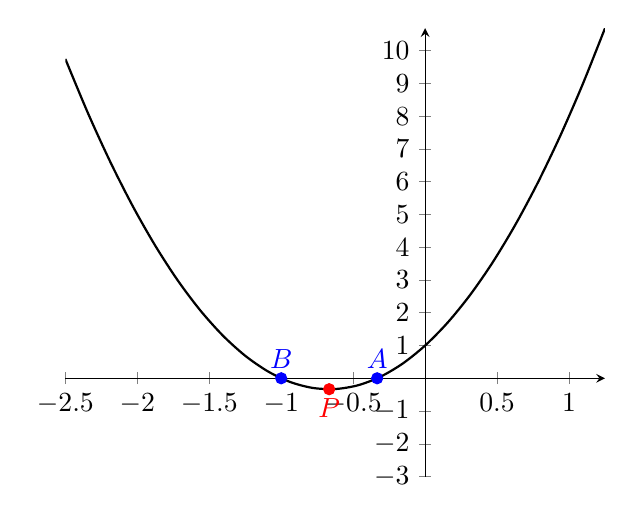
\begin{tikzpicture}
			\begin{axis}[axis lines=middle,ytick distance=1,ymin=-3,xtick distance=.5]
				\addplot[black,thick,smooth,domain=-2.5:1.25] {3 * x^2 + 4 * x + 1};
				\addplot[draw=none,blue,mark=*,nodes near coords={\(B\)}] coordinates {(-1, 0)};
				\addplot[draw=none,blue,mark=*,nodes near coords={\(A\)}] coordinates {(-1/3, 0)};
				\addplot[draw=none,red,mark=*,nodes near coords={\(P\)}] coordinates {(-2/3, -1/3)};
			\end{axis}
		\end{tikzpicture}
	\end{figure}
	\begin{parts}
		\part State the value of the \(y\)-intercept.
		\begin{solution}
			The \(y\)-intercept is \num{1}.
		\end{solution}

		\part Find the coordinates of the points of intersection between the curve and the \(x\)-axis, \(A\) and \(B\).
		\begin{solution}
			\begin{align*}
				3x^{2} + 4x + 1 & = 0                           \\
				(3x + 1)(x + 1) & = 0                           \\
				x               & = -1 \text{ or } -\frac{1}{3}
			\end{align*}
			Hence, the coordinates of the points of intersection between the curve and the \(x\)-axis are \((-1, 0)\) and \(\left(-\frac{1}{3}, 0\right)\).
		\end{solution}
		\begin{subparts}
			\subpart State the range of values of \(x\), for \(3x^{2} + 4x + 1 > 0\).
			\begin{solution}
				\(x < -1\) or \(x > -\dfrac{1}{3}\).
			\end{solution}

			\subpart Hence, find the equation of the line of symmetry.
			\begin{solution}
				\begin{align*}
					x & = \frac{-1 + \left(-\frac{1}{3}\right)}{2} \\
					  & = -\frac{2}{3}
				\end{align*}
			\end{solution}
			\subpart Hence, find the coordinates of the minimum point \(P\).
			\begin{solution}
				\begin{align*}
					y_{P} & = 3x_{P}^{2} + 4x_{P} + 1                                                         \\
					      & = 3 \times \left(-\frac{2}{3}\right)^{2} + 4 \times \left(-\frac{2}{3}\right) + 1 \\
					      & = \frac{4}{3} - \frac{8}{3} + 1                                                   \\
					      & = -\frac{1}{3}
				\end{align*}
				The coordinates of the minimum point \(P\) are \(\left(-\frac{2}{3}, -\frac{1}{3}\right)\).
			\end{solution}

			\subpart Find the area of triangle \(ABP\).
			\begin{solution}
				\begin{align*}
					\text{area of triangle } ABP & = \frac{bh}{2}                             \\
					                             & = \frac{\frac{2}{3} \times \frac{1}{3}}{2} \\
					                             & = \frac{1}{9}
				\end{align*}
			\end{solution}
		\end{subparts}
		\part Find the value of the quadratic expression \(3x^2 + 4x + 1\), when \(x = \frac{1}{3}\).
		\begin{solution}
			\begin{align*}
				3x^2 + 4x + 1 & = 3 \times \left(\frac{1}{3}\right)^2 + 4 \times \left(\frac{1}{3}\right) + 1 \\
				              & = \frac{1}{3} + \frac{4}{3} + 1                                               \\
				              & = \frac{8}{3}
			\end{align*}
		\end{solution}

		\part Write down the straight lines drawn on the same axes to solve the following equations graphically.
		\begin{subparts}
			\subpart \(3x^2 + 4x = 0\)
			\begin{solution}
				\begin{align*}
					3x^2 + 4x     & = 0 \\
					3x^2 + 4x + 1 & = 1 \\
					y             & = 1 \\
				\end{align*}
				\begin{tikzpicture}
					\begin{axis}[width=0.6\pagewidth,axis lines=middle,xtick distance=.5,ytick distance=1,ymin=-1]
						\addplot[black,thick,smooth,domain=-2:1] {3 * x^2 + 4 * x + 1};
						\addplot[red,thick] {1};
					\end{axis}
				\end{tikzpicture}

				\(\therefore x = 0\) or \(x = -1.3\) (\(x = -\frac{4}{3}\) in actuality)
			\end{solution}

			\subpart \(3x^2 + 5x + 1 = 0\)
			\begin{solution}
				\begin{align*}
					3x^2 + 5x + 1 & = 0  \\
					3x^2 + 4x + 1 & = -x \\
					y             & = -x
				\end{align*}
				\begin{tikzpicture}
					\begin{axis}[width=0.6\pagewidth,axis lines=middle,xtick distance=.5,ytick distance=1,ymin=-1]
						\addplot[black,thick,smooth,domain=-2:1] {3 * x^2 + 4 * x + 1};
						\addplot[red,thick] {-x};
					\end{axis}
				\end{tikzpicture}

				\(\therefore x = -1.4\) or \(x = -0.2\) (\(x = \frac{-5 \pm \sqrt{13}}{6}\) in actuality)
			\end{solution}

			\subpart \(3x^2 + 8x - 1 = 0\)
			\begin{solution}
				\begin{align*}
					3x^2 + 8x - 1 & = 0        \\
					3x^2 + 8x + 1 & = 2        \\
					3x^2 + 4x + 1 & = 2 - 4x   \\
					y             & = - 4x + 2 \\
				\end{align*}
				\begin{tikzpicture}
					\begin{axis}[width=0.6\pagewidth,axis lines=middle,xtick distance=.5,ytick distance=1,ymin=-1]
						\addplot[black,thick,smooth,domain=-3:1.5] {3 * x^2 + 4 * x + 1};
						\addplot[red,thick,domain=-3:1] {-4 * x + 2};
					\end{axis}
				\end{tikzpicture}

				\(\therefore x = -2.7\) or \(x = 0.1\) (\(x = \frac{-4 \pm \sqrt{19}}{3}\) in actuality)
			\end{solution}
		\end{subparts}
	\end{parts}

	\question (\textbf{4 May}) If \(5^{78}\) and \(2^{81}\) are multiplied out,
	what is the leading digit of the product? How many zeroes are there in the product?
	\begin{solution}
		\begin{align*}
			5^{78} \times 2^{81} & = \left(2 \times 5\right)^{78} \times 2^3 \\
			                     & = 8 \times 10^{78}
		\end{align*}
		The leading digit of the product is \textbf{8}. The product will have
		\textbf{78} zeroes.
	\end{solution}

	\question (\textbf{5 May}) Given that \(5^3 + 5^3 + 5^3 + 5^3 + 5^3 = 5^x\) and
	\(2^2 + 2^2 = 2^y\), find the value of \(x^y\).
	\begin{solution}
		\begin{align*}
			5^3 + 5^3 + 5^3 + 5^3 + 5^3 & = 5 \times 5^3               \\
			                            & = 5^4                        \\
			x                           & = 4 \label{eq:05051} \tag{1} \\
			2^2 + 2^2                   & = 2 \times 2^2               \\
			                            & = 2^3                        \\
			y                           & = 3 \label{eq:05052} \tag{2} \\
			x^y                         & = 4^3                        \\
			                            & = 64
		\end{align*}
	\end{solution}
\end{questions}
\end{document}
